\documentclass{article}

\usepackage{graphicx}


\title{The Pendula of Atomic Collisions}
\author{Matthew Chilcott}
\date{}


\begin{document}

\maketitle
\thispagestyle{empty}

% - Expand Figure to have two aspects
% - Two references
% - Previous. Now.

% Give the audience a chance ?!?
% Ubiquitous.  In the context of scattering.


% Adds no info:
% Scattering resonances, as present in atomic collisions, are well
% described by a number of successful quantum theories. Many of these
% theories are completely equivalent, though their formulations can
% provide different insights into the underlying physics.

Resonances are ubiquitous in physics, appearing in all manner of
classical and quantum systems. A common example is the increase in the
amplitude of a pendulum driven near its resonant frequency, and
similar resonances occur in a large variety of mechanical, electrical
and optical systems. In atomic scattering, resonances manifest as
drastically enhanced or suppressed scattering at energies near a
quasi-bound state of the system.

We consider the interaction of a Feshbach resonance and a shape
resonance as we have observed in collisions of ultracold
Rubidium. Previously, we have described the interaction in terms of
the avoided crossing of $S$-matrix poles in the complex energy plane
\cite{Chilcott2021A}. Here we elaborate upon the measurements, and
investigate the situation using the paradigm of quantum defect
theory. Quantum defect theory relies on only 6 parameters, yet
provides an adequate model for the physical system. In comparison,
coupled-channels calculations rely on realistic potentials with more
than 40 parameters. We also examine a classical system of two
coupled pendula, which, perhaps surprisingly, provides a good analogy
to the atomic system \cite{ArticleInPrep}.
\vspace{-1em}
\begin{center}
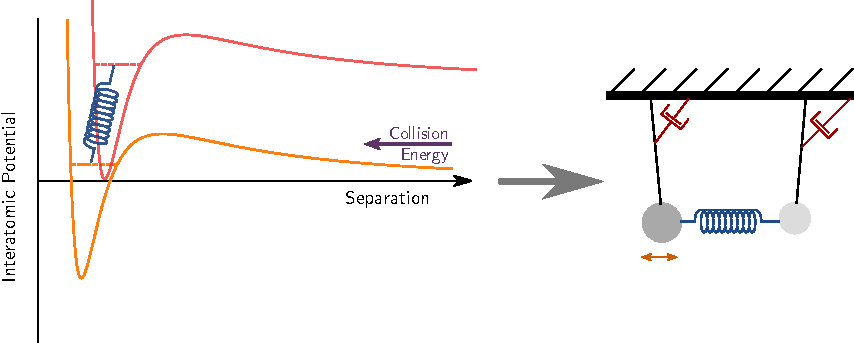
\includegraphics[width=\linewidth]{system.pdf}
\end{center}
\vspace{-3em}
\begin{thebibliography}{1}
\bibitem{Chilcott2021A} Matthew Chilcott, Ryan Thomas, Niels Kj{\ae}rgaard, {\em Experimental observation of the avoided crossing of two $S$-matrix resonance poles in an ultracold atom collider,} arXiv:2103.05278 (2021).

\bibitem{ArticleInPrep} Matthew Chilcott, James F. E. Croft, Ryan Thomas, Niels Kj{\ae}rgaard, {\em Observations and models of interacting collisional resonances,} Manuscript in preparation.

\end{thebibliography}


\end{document}

% LocalWords:  Feshbach ultracold pendula
